\documentclass[10pt,journal,compsoc]{IEEEtran}

\usepackage{amsmath,amssymb,amsfonts}
\usepackage{graphicx}
\usepackage{booktabs}
\usepackage{multirow}
\usepackage{tabularx}
\usepackage{array}
\usepackage{placeins}
\usepackage{url}
\usepackage{dblfloatfix}
\usepackage[ruled,vlined,linesnumbered]{algorithm2e}

\ifCLASSOPTIONcompsoc
  \usepackage[caption=false,font=footnotesize,labelfont=sf,textfont=sf]{subfig}
\else
  \usepackage[caption=false,font=footnotesize]{subfig}
\fi

\ifCLASSOPTIONcompsoc
  \usepackage[nocompress]{cite}
\else
  \usepackage{cite}
\fi

\interdisplaylinepenalty=2500
\providecommand{\Description}[1]{}

% Fine-tune float and spacing hygiene for IEEE Computer Society journal specifications
\setlength{\textfloatsep}{6pt plus 1pt minus 1pt}
\setlength{\floatsep}{5pt plus 1pt minus 1pt}
\setlength{\dbltextfloatsep}{6pt plus 1pt minus 1pt}
\setlength{\dblfloatsep}{5pt plus 1pt minus 1pt}
\setlength{\abovecaptionskip}{2.5pt plus 1pt minus 1pt}
\setlength{\belowcaptionskip}{1pt plus 1pt minus 1pt}

% Compact list spacing
\usepackage{enumitem}
\setlist{nosep,leftmargin=1.2em}

% Bibliography spacing adjustment
\let\oldthebibliography\thebibliography
\let\endoldthebibliography\endthebibliography
\renewenvironment{thebibliography}[1]{%
  \begin{oldthebibliography}{#1}%
    \setlength{\itemsep}{0.8pt plus 0.4pt minus 0.4pt}%
    \setlength{\parsep}{0pt}%
}{%
  \end{oldthebibliography}%
}

\begin{document}
	
\title{CEE-Split: Adaptive Slicing and Scheduling for\\ Cloud-Edge-End Collaborative Rendering}

\author{Anonymous~Author%
\IEEEcompsocitemizethanks{\IEEEcompsocthanksitem The author is with Anonymous University, Anonymous City, Anonymous Country.\protect\\
E-mail: author@anonymous.edu}%
\thanks{Manuscript received Month DD, 202X; revised Month DD, 202X.}}

\markboth{IEEE Transactions on Services Computing,~Vol.~XX, No.~XX,~202X}%
{Author \MakeLowercase{\textit{et al.}}: CEE-Split: Adaptive Slicing and Scheduling for Cloud-Edge-End Collaborative Rendering}

\IEEEtitleabstractindextext{%
\begin{abstract}
Cloud-edge-end (CEE) collaborative rendering can alleviate the computation and energy constraints of standalone extended reality (XR) devices, but practical deployment still faces imbalanced rendering workloads, compression-sensitive recomposition, and coupled scheduling under heterogeneous and time-varying system conditions. We present CEE-Split, a collaborative rendering framework that integrates adaptive task partitioning, depth-aware transmission, and learned online scheduling. Load-Balanced Adaptive Slicing (LBAS) partitions visible scene geometry into Near, Mid, and Far layers according to the cumulative triangle workload, producing approximately balanced scheduling units without splitting individual Renderers. LumaDepth RGB-D Packing (LDP) combines RGB with logarithmic eye-space depth in a single coded frame to support depth-aware terminal composition after lossy video transmission. A reinforcement-learning-based scheduler jointly selects the rendering node, rendering resolution, and transmission rate for each layer using rendering workload and system telemetry. In trace-driven evaluation, LBAS reduces the mean layer-workload coefficient of variation from 0.445 to 0.039. Compared with a training-optimized fixed configuration, CEE-Split reduces mean simulated end-to-end (E2E) latency from 57.84 to 53.89\,ms and estimated terminal energy from 89.03 to 77.40\,mJ, with a 0.54-point decrease in expected VMAF. A physical Unity/WebRTC prototype further validates the workload-balancing effect of LBAS, the robustness of LDP under lossy video coding, and the effectiveness of adaptive CEE rendering under real system conditions.
\end{abstract}

\begin{IEEEkeywords}
Collaborative rendering, deep reinforcement learning, edge computing, extended reality, quality of experience.
\end{IEEEkeywords}}

\maketitle
\IEEEdisplaynontitleabstractindextext
\IEEEpeerreviewmaketitle

% ================================================================
\IEEEraisesectionheading{\section{Introduction}\label{sec:introduction}}
% ================================================================

\IEEEPARstart{E}{xtended reality} (XR) increasingly relies on high-quality interactive rendering, yet standalone devices remain constrained by limited computation capability, thermal budgets, and battery capacity~\cite{lai_furion_2020,chen_you_2025}. Rendering offloading alleviates these limitations by exploiting remote resources~\cite{zhao_virtual_2021,huang_virtual_2023}, while cloud-edge-end (CEE) architectures further combine the complementary capabilities of End devices, Edge servers, and the Cloud~\cite{su_crossport_2026,li_toward_2024}. Effective CEE rendering, however, still requires appropriate task decomposition, reliable recomposition of distributed rendering results, and adaptive resource allocation under heterogeneous system conditions.

Existing collaborative rendering systems employ foreground-background separation~\cite{lai_furion_2020,meng_coterie_2020}, object-level placement~\cite{lu_renderfusion_2023}, image-space partitioning~\cite{corbillon_viewport-adaptive_2017,cantory_image-space_2023}, or client-side reconstruction and reprojection~\cite{ke_collabvr_2023,gao_xrgo_2025}. Although these approaches enable distributed rendering, they generally do not explicitly construct subtasks according to the current frame-level geometric workload. As the viewpoint and visible scene complexity change, workload can become concentrated in one rendering branch, creating a frame-completion straggler. Meanwhile, independently rendered scene subsets must be recomposed after transmission. Color-key boundaries are vulnerable to compression and YUV~4:2:0 chroma subsampling, while directly quantized linear depth provides limited precision for nearby occlusion boundaries. These issues motivate workload-adaptive task partitioning together with a codec-compatible depth representation for terminal recomposition.

Distributed execution further introduces a coupled online scheduling problem. The rendering node, rendering resolution, and transmission rate of each layer jointly affect rendering cost, codec and network delay, terminal energy, and visual quality, while node capability and network conditions vary over time. Rule-based and threshold-driven strategies~\cite{lai_furion_2020,lu_renderfusion_2023} are difficult to tune for these jointly varying factors, motivating adaptive scheduling based on the current rendering workload and observable system state. In this paper, end-to-end latency denotes distributed frame-completion time from rendering through terminal composition; display scan-out and motion-to-photon stages are outside its scope.

To address these challenges, we propose CEE-Split, a CEE collaborative rendering framework integrating adaptive task partitioning, depth-aware transmission, and learned scheduling. Load-Balanced Adaptive Slicing (LBAS) partitions the visible scene into Near, Mid, and Far layers according to cumulative triangle workload, producing approximately balanced scheduling units while keeping each Renderer intact. LumaDepth RGB-D Packing (LDP) combines RGB with logarithmic eye-space depth in a single coded frame to support terminal depth composition after lossy transmission. A Proximal Policy Optimization (PPO) scheduler then selects the rendering node, rendering resolution, and transmission rate for each layer based on the current workload and observable system telemetry, using calibrated latency, expected-quality, and energy models.

The main contributions of this paper are summarized as follows:
\begin{itemize}
	\item \textbf{Adaptive task partitioning:}
	We propose LBAS, which derives Near, Mid, and Far boundaries from cumulative triangle workload rather than fixed depth thresholds, creating approximately balanced and independently schedulable rendering units.
	
	\item \textbf{Compression-robust RGB-D transmission and composition:}
	We design LDP to pack RGB and logarithmic eye-space depth into a single video frame, enabling depth-aware terminal recomposition under conventional lossy video coding.
	
	\item \textbf{Adaptive CEE rendering control:}
	We formulate per-layer node placement, rendering resolution, and transmission-rate selection as a multidiscrete sequential decision problem and train a PPO scheduler using rendering workload and observable system telemetry. We evaluate the resulting framework through both trace-driven experiments and a three-node Web Real-Time Communication (WebRTC) prototype.
\end{itemize}

% ================================================================
\section{Related Work}
\label{sec:related_work}
% ================================================================

\subsection{Collaborative Rendering Architectures}

Early remote-rendering systems migrate the complete graphics pipeline to a server~\cite{shea_cloud_2013,cai_survey_2016,zhao_virtual_2021}. They reduce headset computation but remain sensitive to network delay, bandwidth, and video compression. XRgo~\cite{gao_xrgo_2025} adds client-side reprojection to reduce motion-to-photon latency, but still follows a thin-client model based on a monolithic encoded stream.

Mobile edge computing enables finer edge-client cooperation~\cite{shi_edge_2016,mach_mobile_2017}. Furion and Coterie render latency-sensitive foreground content locally while the server supplies background frames~\cite{lai_furion_2020,meng_coterie_2020}. CollabVR reduces transmission by rendering one eye at the edge and reconstructing the other on the client~\cite{ke_collabvr_2023}. Other systems study foreground-background queues, practical multi-user access networks, and server-rendered volumetric views~\cite{xu_wireless_2025,yeregui_edge_2024,gul_cloud_2020,son_split_2020}.

More recent CEE systems extend cooperation to three tiers. Crossport decomposes rendering and interaction into distributed microservices~\cite{su_crossport_2026}, while Li \emph{et al.} distribute intermediate scene structures and asynchronous asset loading~\cite{li_toward_2024}. Extensive surveys describe the role of edge computing and edge intelligence in immersive services~\cite{xu_edge_2023,tang_systematic_2023}. These architectures support distributed execution and deployment flexibility, but do not explicitly address frame-level geometric workload balance across parallel rendering branches.

\subsection{Graphics Task Decoupling}

Split-rendering systems differ in what they partition. Screen-space methods divide the viewport into tiles, perceptual regions, or mergeable subframes~\cite{corbillon_viewport-adaptive_2017,cantory_image-space_2023}. They exploit viewport predictability or perceptual redundancy, but describe the underlying 3D workload only indirectly and may introduce seams when objects cross boundaries.

Object-based methods assign entities to local or remote renderers~\cite{lu_renderfusion_2023,wen_ar-light_2025,wu_edge-assisted_2024}. RenderFusion~\cite{lu_renderfusion_2023} selects rendering media from polygon count and network conditions; PoClVR~\cite{wu_edge-assisted_2024} distributes point-cloud objects across edge servers. These methods offer finer control than full-frame offloading, but several complex objects can still concentrate load in one spatial region or depth interval. Service-level decomposition improves modularity but likewise does not guarantee balanced frame workloads.

Depth- and stereo-aware systems use fixed foreground-background thresholds or view reconstruction~\cite{lai_furion_2020,meng_coterie_2020,ke_collabvr_2023,chen_you_2025}. A complementary approach partitions the rendering pipeline: distributed hybrid rendering offloads effects such as shadows and ambient occlusion while the client rasterizes the base frame~\cite{tan_dhr_2022,tan_dhrs_2024}, and temporal image-space splitting reprojects intermediate frames from sparse server renders~\cite{steiner_imagebased_2025}. In contrast to partitioning schemes based on predefined spatial or depth boundaries, LBAS derives its depth planes from the current triangle-load distribution.

\subsection{Depth-Aware Streaming and Compositing}

Distributed layer composition requires geometry information in addition to color. Earlier systems preserve depth or visibility through ZIP-compressed depth images or lossless HEVC visibility textures~\cite{chaudhuri_distributed_2008,stengel_lossless_2021}. These representations preserve depth or visibility information with high fidelity, but provide limited flexibility for lossy bitrate adaptation. RenderFusion instead packs replicated 8-bit depth with color for H.264 transmission~\cite{lu_renderfusion_2023}, and prior studies show that packing precision and chroma subsampling materially affect decoded depth~\cite{pece_depth_2011,siekkinen_depth_2023}.

For layer-wise CEE rendering, color-key composition is vulnerable to YUV~4:2:0 chroma subsampling, while linear depth quantization spends much of its finite range on distant geometry. CEE-Split instead packs logarithmic eye-space depth as a grayscale image so that, after RGB-to-YUV conversion, the depth information is primarily carried by the full-resolution luma component, retaining codec bitrate adaptation while allocating more precision to nearby occlusion boundaries.

\subsection{Computation Offloading Strategies}

Rule-based systems such as RenderFusion and Crossport select rendering media or service placement with predefined heuristics~\cite{lu_renderfusion_2023,su_crossport_2026}. Such rules are effective in their target regimes but become difficult to tune when rendering load, bandwidth, codec delay, and heterogeneous node capacity vary jointly.

Learning-based control has been applied to adaptive streaming and general computation offloading~\cite{schulman_proximal_2017,mao_neural_2017,huang_deep_2020,tang_deep_2025,yang_dqn_2022}. In edge and VR settings, prior work combines actor-critic learning with recurrent models for dynamic task scheduling, jointly optimizes foveated rendering and radio resources, or manages tile placement and execution queues~\cite{tuli_dynamic_2022,nyamtiga_adaptive_2024,xu_wireless_2025,saha_deep_2026}. These studies show that learning-based control can adapt coupled decisions under time-varying conditions.

CEE-Split considers multiple rendering layers whose placement, resolution, and rate decisions are coupled through rendering, codec, network, terminal energy, and quality effects. We formulate layer-wise scheduling as a multidiscrete control problem and incorporate a lightweight expected-quality proxy into a deadline-aware reward.

% ================================================================
\section{CEE-Split Design}
\label{sec:design}
% ================================================================

\subsection{Task Slicing}

Effective CEE collaboration requires rendering tasks that are sufficiently fine-grained for dynamic scheduling while avoiding severe workload imbalance among parallel branches. Fixed depth thresholds do not provide this property because geometric complexity is generally distributed non-uniformly along the viewing direction. CEE-Split therefore employs LBAS to construct three independently schedulable Near, Mid, and Far layers according to the current geometric workload distribution.

For slicing update $t$, let $\mathcal{O}_t$ denote the set of Renderers whose axis-aligned bounds intersect the current camera frustum. A Renderer represents one drawable scene component with its own geometry and bounds and is treated as the atomic slicing unit; LBAS does not geometrically clip a Renderer across layers. For each Renderer $o_k\in\mathcal{O}_t$, we use its triangle count $w_{k,t}$ as a lightweight geometry-side workload proxy and define its depth key $z_{k,t}$ as the minimum distance from the camera to its axis-aligned bounding box. The resulting triangle-weighted depth distribution is
\begin{equation}
	\Lambda_t(z)=\sum_{o_k\in\mathcal{O}_t}w_{k,t}\,\delta(z-z_{k,t}),
\end{equation}
where $\delta(\cdot)$ is the Dirac delta function. The cumulative geometric workload in $[z_a,z_b]$ is
\begin{equation}
	L_t(z_a,z_b)=\int_{z_a}^{z_b}\Lambda_t(z)\,dz
	=\sum_{\substack{o_k\in\mathcal{O}_t\\z_a\le z_{k,t}\le z_b}}w_{k,t}.
\end{equation}

Let $W_t=\sum_{o_k\in\mathcal{O}_t}w_{k,t}$ be the total visible geometric workload. LBAS orders the Renderers by their depth keys and accumulates triangle counts along the viewing direction. With default target fractions $\rho_{\mathrm{N}}=\rho_{\mathrm{M}}=\rho_{\mathrm{F}}=1/3$, the unsmoothed Near and Mid boundaries are
\begin{align}
	d_t^{*,\mathrm{N}}&=\min\{z\mid L_t(0,z)\ge \rho_{\mathrm{N}}W_t\},\\
	d_t^{*,\mathrm{M}}&=\min\{z\mid L_t(0,z)\ge(\rho_{\mathrm{N}}+\rho_{\mathrm{M}})W_t\}.
\end{align}

\begin{figure}[t]
	\centering
	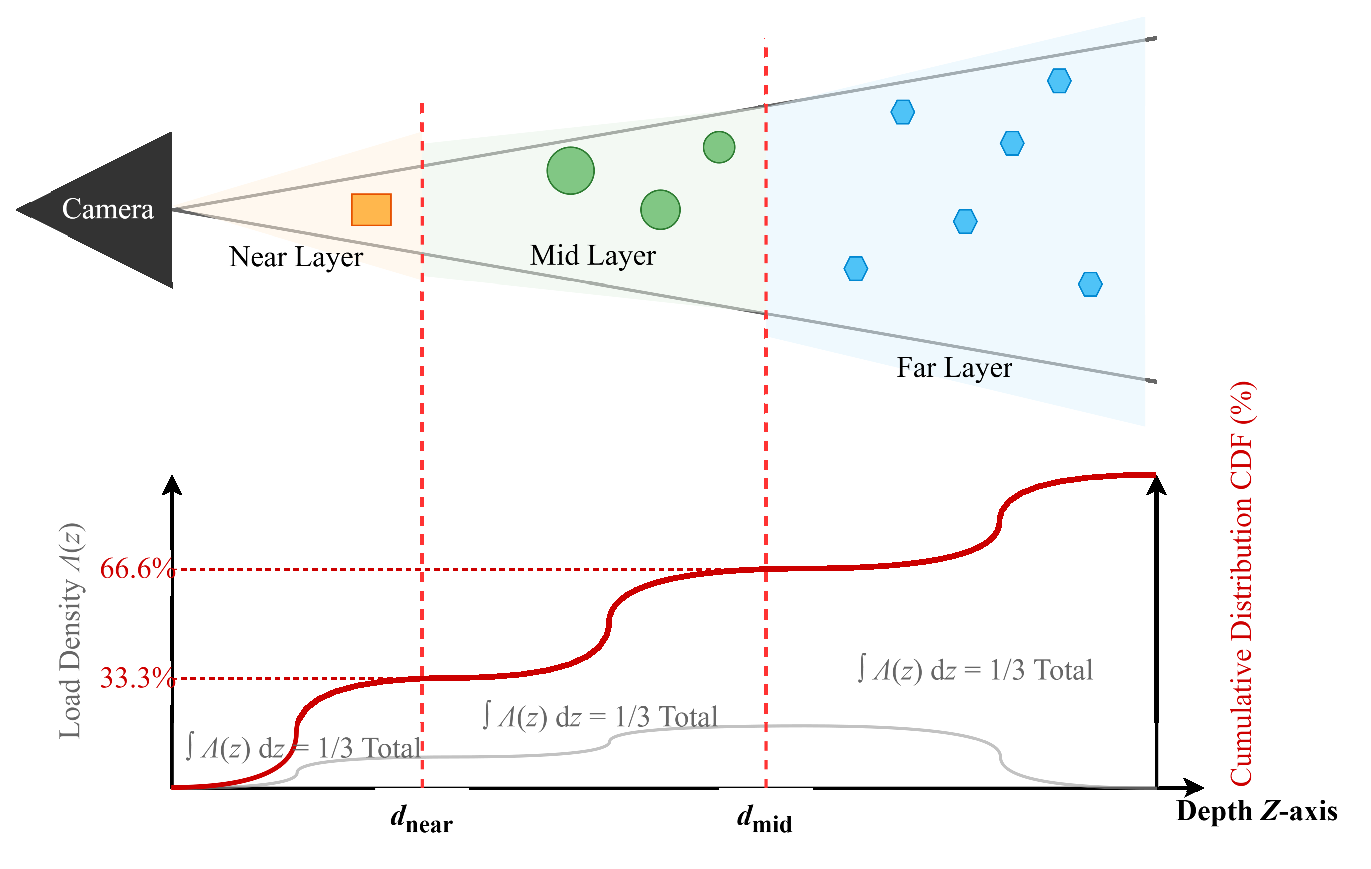
\includegraphics[width=0.90\columnwidth]{assets/figures/design/fig_lbas_principle.eps}
	\caption{Illustration of LBAS. Visible Renderers are ordered along camera depth, and the Near and Mid boundaries are placed near the one-third and two-thirds quantiles of cumulative triangle workload.}
	\label{fig:lbas}
\end{figure}

As illustrated in Fig.~\ref{fig:lbas}, the two boundaries approximately place one-third of the visible triangle workload in each layer. Because Renderers remain intact, exact equality is not guaranteed. The equal targets create well-conditioned scheduling units; they do not prescribe equal work to heterogeneous End, Edge, and Cloud nodes, whose assignments are selected by the scheduler.

To suppress abrupt boundary motion as the camera or scene objects move, the applied boundary $d_t^b$, $b\in\{\mathrm{N},\mathrm{M}\}$, is temporally smoothed:
\begin{equation}
	d_t^b=(1-\alpha_{\mathrm{smooth}})d_{t-1}^b
	+\alpha_{\mathrm{smooth}}d_t^{*,b}.
\end{equation}
The prototype updates the slicing state every 0.2\,s and sets $\alpha_{\mathrm{smooth}}=0.5$. Membership uses strict depth comparisons: a Renderer with depth exactly equal to an applied boundary is assigned to the farther adjacent layer. Smoothing intentionally trades exact instantaneous balance for temporal stability, while the scheduler handles the remaining workload asymmetry.

\subsection{Layer Transmission and Depth Composition}
\label{sec:compositing}

After scheduling, each rendering node processes its assigned layer set and produces one node-level color and depth output. Each active remote node transmits one RGB-D stream to the End node, where remote outputs are combined with the locally rendered result. To support depth-aware recomposition under lossy video coding, we design LDP.

LDP packs RGB and its corresponding depth map into one double-height frame. For an RGB viewport of size $W\times H$, the upper half stores RGB and the lower half stores grayscale depth. Color and depth consequently share one coded-frame timestamp. Compared with chroma-key-based layer identification, this approach avoids making composition depend on chroma values that are spatially subsampled and perturbed by YUV~4:2:0 coding. It also avoids the inefficient allocation of 8-bit precision produced by directly quantizing linear depth over a large range.

Let $n$ and $f$ denote the camera near and far clipping planes, respectively, and let $z_{\mathrm{eye}}$ denote eye-space depth. LDP maps depth to
\begin{equation}
	d=\frac{\log_2(z_{\mathrm{eye}}/n)}{\log_2(f/n)}.
	\label{eq:log_depth}
\end{equation}
Logarithmic mapping allocates finer quantization resolution to smaller depths and therefore helps preserve nearby occlusion boundaries. The normalized value is written as grayscale $(d,d,d)$ in the lower half of the packed frame. After RGB-to-YUV conversion, this grayscale signal is primarily carried by the full-resolution luminance component rather than the subsampled chroma components. At the receiver, a decoded normalized depth $d_i$ from node $i$ is reconstructed as
\begin{equation}
	\widehat z_i=n\,2^{d_i\log_2(f/n)}=n\left(\frac{f}{n}\right)^{d_i}.
\end{equation}

Algorithm~\ref{alg:compositing_pipeline} summarizes node-level packing, depth recovery, and the minimum-depth composition performed at the terminal.
The prototype sets $\theta_{\mathrm{bg}}=0.995$, allowing for codec perturbations around the ideal far-plane sentinel $d=1$. The End node selects, among the active node-level RGB-D outputs, the valid sample with the smallest reconstructed eye-space depth.

\begin{algorithm}[t]
	\caption{Node-Level LDP and Minimum-Depth Composition}
	\label{alg:compositing_pipeline}
	\KwIn{Active node-level RGB-D outputs indexed by $i$; global clip planes $(n,f)$}
	\KwOut{Composited final viewport $\mathbf{C}_{\mathrm{final}}$}
	\BlankLine
	\tcc{Phase 1: one packed stream per active remote node}
	\For{each active remote node $i$}{
		\For{$0\le x<W$ and $0\le y<H$}{
			$\mathrm{Frame}_i[x,y] \gets \mathrm{SampleColor}(i,\,x,\,y)$\;
			$z_{\mathrm{eye}} \gets \mathrm{LinearEyeDepth}(\mathrm{SampleDepth}(i,\,x,\,y))$\;
			$d \gets \log_2(z_{\text{eye}} / n) / \log_2(f / n)$\;
			$\mathrm{Frame}_i[x,y+H] \gets (d,\,d,\,d)$\;
		}
		Encode and transmit $\mathrm{Frame}_i$ through WebRTC\;
	}
	\BlankLine
	\tcc{Phase 2: compose node-level outputs}
	$\widehat z_*\gets\infty$;\enskip $\mathbf{C}_{\mathrm{final}}\gets\mathbf{C}_{\mathrm{bg}}$\;
	\For{each active rendering node $i$}{
		$\mathrm{Frame}_i\gets\mathrm{DecodedOrLocalFrame}(i)$\;
		$\mathbf{C}_i\gets\mathrm{UpperHalf}(\mathrm{Frame}_i)$;\enskip
		$d_i\gets\mathrm{LowerHalf}(\mathrm{Frame}_i).\mathrm{red}$\;
		\eIf{$d_i\ge\theta_{\mathrm{bg}}$}{
			$\widehat z_i\gets\infty$\;
		}{
			$\widehat z_i\gets n\cdot2^{d_i\log_2(f/n)}$\;
		}
		\lIf{$\widehat z_i<\widehat z_*$}{$(\widehat z_*,\mathbf{C}_{\mathrm{final}})\gets(\widehat z_i,\mathbf{C}_i)$}
	}
	\Return{$\mathbf{C}_{\mathrm{final}}$}
\end{algorithm}

\subsection{Collaborative Framework}

The proposed CEE-Split integrates adaptive task slicing and depth-aware transmission into a three-tier rendering framework. At each scheduling step, the End node applies LBAS to partition visible geometry into Near, Mid, and Far layers, which form the basic scheduling units. Based on the current workload and system conditions, the scheduler determines the rendering node, rendering resolution, and transmission configuration for each layer. Fig.~\ref{fig:architecture} illustrates the resulting architecture. Scene assets are synchronized before execution, while the End node performs slicing, scheduling, control dispatch, and final frame reconstruction. The deployed experiments use a fixed pretrained actor without online policy updates.

After scheduling, active nodes render their assigned layers in parallel. Each remote node packs its node-level RGB-D output with LDP and transmits one stream to the End device, where received streams are decoded and combined with the locally rendered result through depth-aware composition. Fig.~\ref{fig:pipeline} illustrates this execution pipeline. Since rendering branches proceed concurrently, frame completion is determined by the slowest active branch followed by terminal composition.

\begin{figure*}[!t]
	\centering
	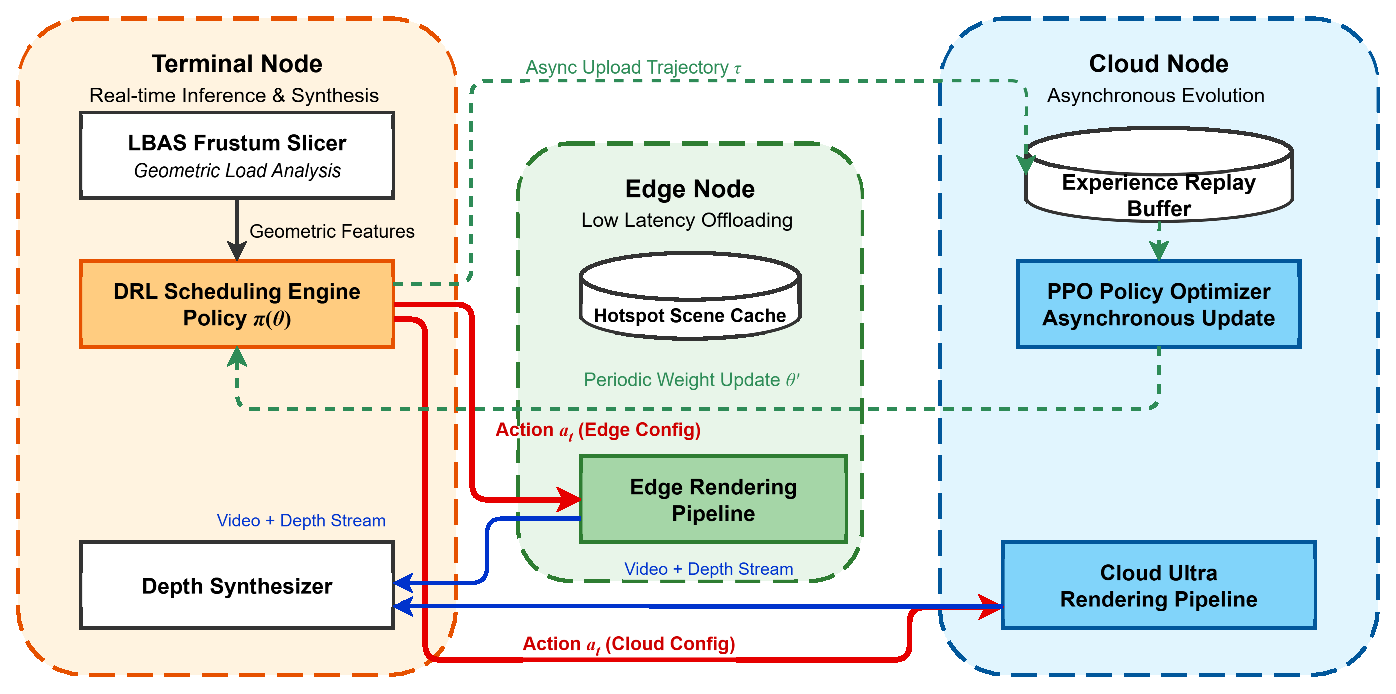
\includegraphics[width=0.78\textwidth]{assets/figures/design/fig_macro_architecture.eps}
	\caption{CEE macro architecture.}
	\label{fig:architecture}
\end{figure*}

\begin{figure*}[!t]
	\centering
	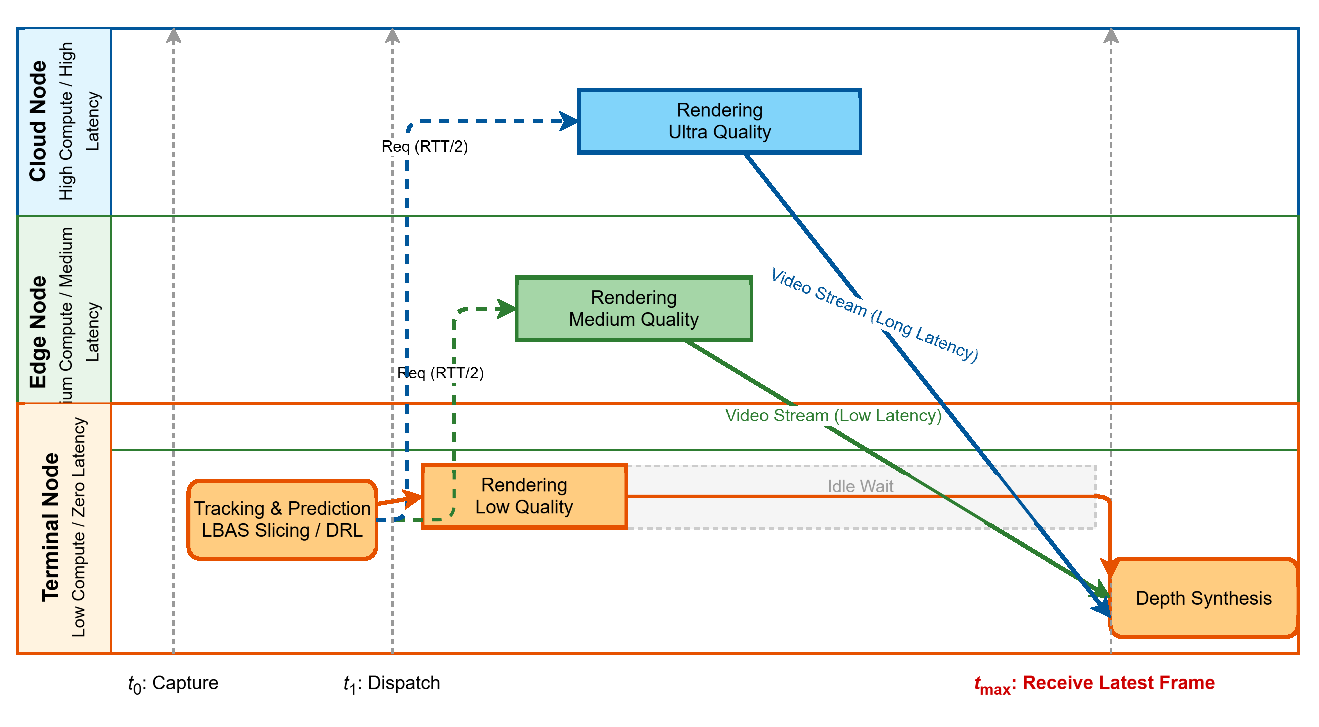
\includegraphics[width=0.80\textwidth]{assets/figures/design/fig_pipeline_timing.eps}
	\caption{Parallel timing of the distributed rendering pipeline.}
	\label{fig:pipeline}
\end{figure*}

% ================================================================
\section{System Model}
\label{sec:system_model}
% ================================================================

To support policy training in the trace-driven environment, we model the system outcome associated with each scheduling configuration. Given the layer-to-node assignment, rendering resolution, and transmission-rate decisions, the model estimates rendering, codec, and network latency, end-to-end frame-completion time, expected visual quality, and terminal energy consumption.
	
\subsection{Rendering Workload Model}
\label{sec:workload_model}

Let $\mathcal{K}=\{\mathrm{Near},\mathrm{Mid},\mathrm{Far}\}$ be the layer set and $\mathcal{N}=\{\mathrm{End},\mathrm{Edge},\mathrm{Cloud}\}$ the set of rendering nodes. For layer $k$ in frame $t$, $N_{k,t}\in\mathcal{N}$ is the execution node decision and $D_{k,t}$ is its triangle count. The resolution action index $U_{k,t}\in\mathcal{U}=\{0,1,2,3,4\}$ and network rate action index $B_{k,t}\in\mathcal{B}=\{0,1,2,3,4\}$ are selected independently. The rendering resolution of layer $k$ is $R^{render}_{k,t}=\mathcal{R}(U_{k,t})$, measured in pixels. If $\mathcal{K}_{i,t}=\{k\mid N_{k,t}=i\}$ is the set of layers assigned to node $i$, the node-level model aggregates their geometry while retaining the rendering resolution of each layer. Before packing, the layer outputs are scaled to a common RGB-D canvas. Because one node produces one packed stream, its transmission resolution and target rate use the highest indices requested by its assigned layers:
\begin{align}
	D_{i,t}&=\sum_{k\in\mathcal{K}_{i,t}}D_{k,t}, &
	U^{tx}_{i,t}&=\max_{k\in\mathcal{K}_{i,t}}U_{k,t},\\
	R^{tx}_{i,t}&=\mathcal{R}(U^{tx}_{i,t}), &
	B^{tx}_{i,t}&=\max_{k\in\mathcal{K}_{i,t}}B_{k,t},\\
	R^{pack}_{i,t}&=2R^{tx}_{i,t}.
\end{align}
Here $R^{tx}_{i,t}$ is the RGB viewport pixel count of the node-level transmission canvas, and $R^{pack}_{i,t}$ is the physical pixel count of its double-height LDP frame. Thus, a nominal $W\times H$ transmission resolution is encoded as $W\times2H$. The rate action is ignored for a locally rendered layer because it is not transmitted. Following the vertex-fragment decomposition in~\cite{xu_wireless_2025}, rendering time is modeled by separate geometry and pixel terms:
\begin{equation}
	T^{render}_{i,t}=
	\frac{a_{D,i}D_{i,t}+a_{R,i}
	\sum_{k\in\mathcal{K}_{i,t}}R^{render}_{k,t}}{c_{i,t}}
	\quad [\mathrm{ms}],
	\label{eq:render_time}
\end{equation}
for $\mathcal{K}_{i,t}\ne\varnothing$, where $a_{D,i}$ and $a_{R,i}$ are the node-specific triangle and pixel coefficients, respectively, and $c_{i,t}$ is a dimensionless relative-capacity multiplier. We define $c_{i,t}=1$ as the calibrated baseline of node $i$; values above or below one represent proportional performance improvement or degradation, respectively. The triangle count, resolution, and rendering time are measured while roaming through different scenes, and the triangle-to-pixel cost ratio is obtained from these measurements by least-squares linear regression. Keeping this fitted ratio, the coefficient pair of each node is calibrated at $c_{i,t}=1$ against its measured rendering time under the common reference workload. The coefficients $a_{D,i}$ and $a_{R,i}$ are expressed in ms/triangle and ms/pixel, respectively. All coefficients are fixed during training and evaluation, while $c_{i,t}$ models runtime variation. The resulting calibrated values are listed in Table~\ref{tab:render_coefficients}.

\begin{table}[t]
	\centering
	\caption{Calibrated Rendering Parameters Used in Simulation}
	\label{tab:render_coefficients}
	\footnotesize
	\setlength{\tabcolsep}{3pt}
	\renewcommand{\arraystretch}{1.05}
	\begin{tabular*}{\columnwidth}{@{\extracolsep{\fill}}lcccc@{}}
		\toprule
		\textbf{Node} & $\boldsymbol{a_{D,i}}$ & $\boldsymbol{a_{R,i}}$ &
		$\boldsymbol{c_{i,t}}$ \textbf{(train)} & $\boldsymbol{T_{ref}}$ \textbf{(ms)} \\
		\midrule
		End   & $2.6857\!\times\!10^{-5}$ & $2.1699\!\times\!10^{-5}$ & $[0.5,1.5]$ & 60.0 \\
		Edge  & $1.7904\!\times\!10^{-6}$ & $1.4466\!\times\!10^{-6}$ & $[0.7,1.3]$ & 4.0 \\
		Cloud & $1.1190\!\times\!10^{-6}$ & $9.0413\!\times\!10^{-7}$ & $[0.8,1.2]$ & 2.5 \\
		\bottomrule
	\end{tabular*}
	\par\smallskip
	\raggedright\scriptsize The reference workload contains 558.7k triangles and
	1920$\times$1080 pixels. $T_{ref}$ is its measured rendering time at $c_{i,t}=1$;
	the coefficient pairs are fitted at this calibrated baseline.\par
\end{table}

\subsection{Codec and Transmission Model}
\label{sec:codec_transmission}

Each rate action $B\in\mathcal{B}$ maps to a WebRTC target bitrate $b(B)$ and a quantization parameter (QP) calibration label $QP(B)$, as listed in Table~\ref{tab:qp_rate_map}. The target bitrate determines the transmission load in the trace-driven environment, whereas $QP(B)$ serves only as an offline calibration coordinate for the expected-VMAF proxy in Section~\ref{sec:quality_energy}. WebRTC performs rate control internally, so the scheduler does not directly control the actual per-frame QP.

At frame rate $F=60$\,fps, the per-frame payload used by the trace-driven simulator for an active remote node is
\begin{equation}
	S^{sim}_{i,t}=\frac{b(B^{tx}_{i,t})}{F}
	\quad[\mathrm{Mbit/frame}].
	\label{eq:payload}
\end{equation}
The physical prototype instead applies the selected target bitrate directly through WebRTC. With available bandwidth $BW_{i,t}$ in Mbit/s and round-trip time (RTT) $\tau^{RTT}_{i,t}$ in ms, remote transport time is
\begin{equation}
	T^{net}_{i,t}=1000\frac{S^{sim}_{i,t}}{BW_{i,t}}+\frac{\tau^{RTT}_{i,t}}{2}.
	\label{eq:network_time}
\end{equation}
We denote the serialization term (the first term in Equation~\ref{eq:network_time}) by $T^{ser}_{i,t}$. The RTT term approximates one-way propagation delay. Resolution-dependent codec and composition times are affine:
\begin{align}
	T^{enc}_{i,t}&=\varepsilon_0+\varepsilon_1R^{pack}_{i,t},\\
	T^{dec}_{i,t}&=\zeta_0+\zeta_1R^{pack}_{i,t},\\
	T^{comp}_{t}&=\chi_0+\chi_1R^{display}_{t},
	\label{eq:codec_comp_time}
\end{align}
where $T^{dec}_{i,t}$ denotes terminal decoding time for the stream received from node $i$, and $R^{display}_{t}$ is the terminal composition resolution in pixels. The coefficients are fitted from stage times measured at multiple resolutions. Composition remains approximately 0.1\,ms over the tested resolutions and is therefore modeled as a constant. The fitted values are listed in Table~\ref{tab:codec_coefficients}.

\begin{table}[t]
	\centering
	\caption{Mapping Between Network Rate Levels, WebRTC Target Bitrates, and QP Calibration Labels}
	\label{tab:qp_rate_map}
	\footnotesize
	\renewcommand{\arraystretch}{1.05}
	\begin{tabular*}{\columnwidth}{@{\extracolsep{\fill}}lccccc@{}}
		\toprule
		\textbf{Rate level} & 0 & 1 & 2 & 3 & 4 \\
		\midrule
		\textbf{Target bitrate (Mbit/s)} & 1 & 2.5 & 5 & 8 & 10 \\
		\textbf{QP calibration label} & 40 & 34 & 28 & 24 & 20 \\
		\bottomrule
	\end{tabular*}
\end{table}

\begin{table}[t]
	\centering
	\caption{Fitted Codec-Time Coefficients Used in Simulation}
	\label{tab:codec_coefficients}
	\footnotesize
	\setlength{\tabcolsep}{4.5pt}
	\renewcommand{\arraystretch}{1.05}
	\begin{tabular*}{\columnwidth}{@{\extracolsep{\fill}}lccc@{}}
		\toprule
		\textbf{Stage} & \textbf{Intercept (ms)} &
		\textbf{Slope (ms/pixel)} & \textbf{Applied nodes} \\
		\midrule
		Encoding & $\varepsilon_0=0.5$ & $\varepsilon_1=2.5\times10^{-7}$ & Edge, Cloud \\
		Decoding & $\zeta_0=1.0$ & $\zeta_1=2.5\times10^{-7}$ & Edge, Cloud \\
		Composition & $\chi_0=0.1$ & $\chi_1=0$ & End \\
		\bottomrule
	\end{tabular*}
\end{table}

\subsection{End-to-End Latency Model}

The completion time of active node branch $i$ is
\begin{equation}
	H_{i,t}=
	\begin{cases}
		T^{render}_{i,t}, & i=\mathrm{End},\\
		T^{render}_{i,t}+T^{enc}_{i,t}\\
		\quad +\,T^{net}_{i,t}+T^{dec}_{i,t},
		& i\in\{\mathrm{Edge},\mathrm{Cloud}\}.
	\end{cases}
	\label{eq:branch_latency}
\end{equation}
All active branches execute concurrently, so the end-to-end (E2E) latency is
\begin{equation}
	L_{final,t}=\max_{i:\mathcal{K}_{i,t}\neq\emptyset}H_{i,t}+T^{comp}_{t}
	\quad [\mathrm{ms}].
	\label{eq:e2e_latency}
\end{equation}

\subsection{Visual Quality Proxy and Terminal Energy Model}
\label{sec:quality_energy}

We use Video Multimethod Assessment Fusion (VMAF) as the full-reference perceptual metric for offline calibration. Direct VMAF evaluation is unsuitable for per-frame scheduling because it requires a reference frame and incurs substantial computation. We therefore use a lightweight multilayer perceptron (MLP) to estimate the configuration-level expected VMAF associated with each layer. For an active remote node, $QP^{tx}_{i,t}=QP(B^{tx}_{i,t})$. The effective calibration label of layer $k$ is
\begin{equation}
	QP^{eff}_{k,t}=\begin{cases}
		QP(4)=20, & N_{k,t}=\mathrm{End},\\
		QP^{tx}_{N_{k,t},t}, & N_{k,t}\in\{\mathrm{Edge},\mathrm{Cloud}\},
	\end{cases}
	\label{eq:effective_qp}
\end{equation}
where a local layer uses the highest-quality label only as a proxy coordinate because it is not video encoded. The proxy estimate is
\begin{equation}
	\widehat V_{k,t}=f_{\psi}\!\left(R^{render}_{k,t},QP^{eff}_{k,t}\right).
	\label{eq:vmaf_proxy}
\end{equation}
The MLP is calibrated from VP9 samples; its dataset and held-out accuracy are reported in Section~\ref{sec:training_setup}. Throughout the remainder of this paper, $\widehat V_{k,t}$ and aggregates derived from it denote expected VMAF, not directly measured received-stream VMAF.

Terminal energy combines local rendering, radio-active communication, and baseline system-on-chip (SoC) activity:
\begin{equation}
\begin{aligned}
	E_{total,t}=&\,P_{\mathrm{GPU}}T^{render}_{\mathrm{End},t}
	+P_{\mathrm{radio}}\!\left(T^{ser}_{\mathrm{Edge},t}+T^{ser}_{\mathrm{Cloud},t}\right)\\
	&+\,P_{\mathrm{base}}L_{final,t}\quad[\mathrm{mJ}],
\end{aligned}
	\label{eq:energy_model}
\end{equation}
where time is in ms and power is in W, so each product is in mJ.
$P_{\mathrm{GPU}}=5.0$\,W, $P_{\mathrm{radio}}=1.5$\,W, and $P_{\mathrm{base}}=1.0$\,W are simulation parameters for local GPU rendering, radio-active reception and control traffic, and baseline terminal activity, respectively. Energy is evaluated only in the trace-driven environment.

% ================================================================
\section{Scheduling Method}
\label{sec:scheduling_method}
% ================================================================

Based on the system model in Section~\ref{sec:system_model}, CEE-Split performs per-frame scheduling of layer-to-node assignment, rendering resolution, and transmission rate. Motivated by prior deep reinforcement learning (DRL)-based online task scheduling in dynamic, heterogeneous, and stochastic edge-cloud environments~\cite{tuli_dynamic_2022,yang_dqn_2022}, we formulate this sequential process as a Markov decision process (MDP) and employ PPO~\cite{schulman_proximal_2017} to learn an adaptive scheduling policy.

\subsection{MDP Formulation}
\label{sec:mdp}

We model the scheduling process as $\mathcal{M}=(\mathcal{S},\mathcal{A},P,R,\gamma)$, where $\mathcal{S}$ and $\mathcal{A}$ denote the state and action spaces, $P(\mathbf{s}_{t+1}\mid\mathbf{s}_t,\mathbf{a}_t)$ is the transition kernel, $R$ is the immediate reward, and $\gamma\in[0,1)$ is the discount factor. At each frame, the policy observes the current rendering workload, network and pipeline telemetry, together with recent scheduling outcomes, and selects the rendering and transmission configuration for the three layers. Fig.~\ref{fig:mdp} summarizes the resulting interaction between the policy and the rendering environment.

\begin{figure}[t]
	\centering
	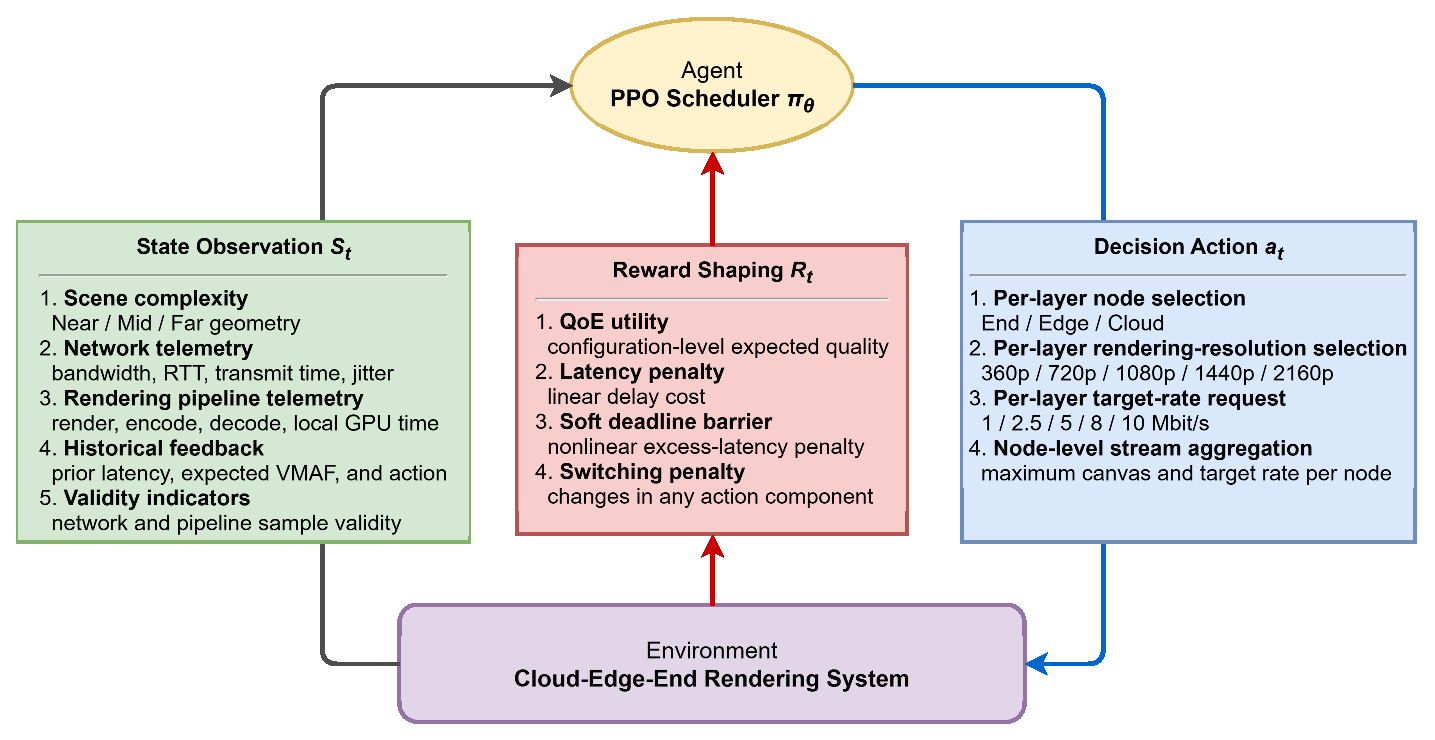
\includegraphics[width=0.88\columnwidth]{assets/figures/design/fig_drl_mdp_decoupled.eps}
	\caption{Interaction among the state, action, and environment in the learning agent.}
	\label{fig:mdp}
\end{figure}

\subsubsection{State Space}

The policy uses the following 36-dimensional observation vector:
\begin{equation}
	\mathbf{s}_t = [\mathbf{g}_t,\mathbf{n}^{c}_t,\mathbf{n}^{e}_t,
	\mathbf{p}^{c}_t,\mathbf{p}^{e}_t,\mathbf{p}^{l}_t,
	\boldsymbol{\ell}_{t-1},\mathbf{v}_{t-1},\mathbf{a}_{t-1}],
\end{equation}
where superscripts $c$, $e$, and $l$ denote Cloud, Edge, and local End, respectively. The workload vector $\mathbf{g}_t\in\mathbb{R}^{3}$ contains the log-scaled triangle counts of the Near, Mid, and Far layers. For each remote node $x\in\{c,e\}$, the five-dimensional network-state vector $\mathbf{n}^{x}_t=[BW_x,RTT_x,T^{ser}_x,J_x,I_x]$ contains normalized bandwidth, round-trip time, the measured serialization time, jitter, and a telemetry validity indicator. The pipeline vectors $\mathbf{p}^{c}_t$ and $\mathbf{p}^{e}_t$ contain the measured rendering, encoding, and decoding times of the corresponding remote branches, while $\mathbf{p}^{l}_t$ contains local GPU rendering time and its validity indicator. To expose recent scheduling outcomes to the policy, $\boldsymbol{\ell}_{t-1}\in\mathbb{R}^{3}$ records the previous per-layer latency, $\mathbf{v}_{t-1}\in\mathbb{R}^{3}$ records the previous per-layer expected VMAF, and $\mathbf{a}_{t-1}\in\mathbb{R}^{9}$ records the previous scheduling action. The validity indicators distinguish unavailable telemetry from genuinely low measured values.

\subsubsection{Action Space}
\label{sec:action_space}

At each frame, the scheduler selects the rendering node, rendering resolution, and transmission-rate level for each of the three layers. The resulting nine-dimensional multidiscrete action is
\begin{equation}
\begin{aligned}
	\mathbf{a}_t = [&N_{\mathrm{near},t},\, U_{\mathrm{near},t},\, B_{\mathrm{near},t},\\
	&N_{\mathrm{mid},t},\, U_{\mathrm{mid},t},\, B_{\mathrm{mid},t},\\
	&N_{\mathrm{far},t},\, U_{\mathrm{far},t},\, B_{\mathrm{far},t}],
\end{aligned}
\end{equation}
where $N_{k,t} \in \{0\!=\!\text{End},\, 1\!=\!\text{Edge},\, 2\!=\!\text{Cloud}\}$ selects the rendering node for layer $k$. The rendering-resolution index $U_{k,t}$ maps to $\{640\!\times\!360,1280\!\times\!720,1920\!\times\!1080,2560\!\times\!1440,3840\!\times\!2160\}$, while $B_{k,t}$ independently maps to the WebRTC target rates and QP calibration labels, as shown in Table~\ref{tab:qp_rate_map}. The corresponding per-frame payload is determined from the selected target bitrate as described in Section~\ref{sec:codec_transmission}. Decoupling resolution and rate allows the scheduler to control rendering pixel workload and the transmission-rate/quality trade-off independently rather than being restricted to fixed resolution-rate pairs.

For layers assigned to the same node, the node-level transmission configuration follows the aggregation rule in Section~\ref{sec:workload_model}, while the rate action of a locally rendered layer is ignored. The unfactorized action space contains $(3\times5\times5)^3=421{,}875$ possible tuples. Instead of representing them with a single categorical distribution, the policy uses nine categorical heads with a shared feature encoder. This factorization substantially reduces the output dimensionality while preserving the complete nine-component scheduling action.

\subsubsection{Reward Function}
\label{sec:reward}

The scheduler balances expected visual quality, frame-completion latency, terminal energy, and temporal stability of the scheduling decisions. As illustrated in Fig.~\ref{fig:degradation}, reducing the resolution of the Near layer produces more noticeable foreground degradation than applying a comparable reduction to distant content. We therefore use fixed depth weights $[\omega_{\mathrm{Near}},\omega_{\mathrm{Mid}},\omega_{\mathrm{Far}}]=[0.50,0.35,0.15]$ to emphasize nearer content. Then the depth-weighted expected-VMAF utility is
\begin{equation}
	V_{pw,t}=\sum_{k\in\mathcal{K}}\omega_k\widehat V_{k,t},
	\label{eq:vpw_model}
\end{equation}
where $\widehat V_{k,t}$ is the expected VMAF defined in Section~\ref{sec:quality_energy}. We define the amount by which the frame-completion latency exceeds the 100\,ms soft target as $\Delta L_t=\max(0,L_{final,t}-100)$. The quality, latency, and energy reward terms are defined as follows:
\begin{align}
	r_{quality,t} &= 0.15(V_{pw,t}-50), \label{eq:rqual}\\
	r_{latency,t} &= -0.03L_{final,t} \nonumber\\
	&\quad -\mathbb{I}(\Delta L_t>0)
	\left(2+0.08\Delta L_t+0.002\Delta L_t^2\right), \label{eq:rlat}\\
	r_{energy,t} &= -0.004E_{total,t}.
\end{align}
The additional nonlinear term in Equation~\ref{eq:rlat} increasingly penalizes latency once the 100\,ms soft target is exceeded, where the target acts as a soft latency objective rather than a hard feasibility constraint. Besides, to discourage frequent configuration changes, we further define
\begin{equation}
	r_{switch,t}=c_{switch}\mathbb{I}\!\left(\mathbf{a}_t\neq\mathbf{a}_{t-1}\right),
	\qquad c_{switch}=0.2.
	\label{eq:rswitch}
\end{equation}
The final reward is
\begin{equation}
	R_t=\operatorname{clip}
	(r_{quality,t}+r_{latency,t}+r_{energy,t}-r_{switch,t},-30,15).
	\label{eq:reward}
\end{equation}

\begin{figure*}[!t]
	\centering
	\subfloat[Baseline\label{fig:deg_a}]{%
		\includegraphics[width=0.215\textwidth]{assets/figures/quality/fig_visual_a.png}%
	}%
	\hfil
	\subfloat[Near degraded\label{fig:deg_b}]{%
		\includegraphics[width=0.215\textwidth]{assets/figures/quality/fig_visual_b.png}%
	}%
	\hfil
	\subfloat[Mid degraded\label{fig:deg_c}]{%
		\includegraphics[width=0.215\textwidth]{assets/figures/quality/fig_visual_c.png}%
	}%
	\hfil
	\subfloat[Far degraded\label{fig:deg_d}]{%
		\includegraphics[width=0.215\textwidth]{assets/figures/quality/fig_visual_d.png}%
	}
	\caption{Perceptual effect of layer-wise resolution degradation. Degrading the Near layer noticeably blurs foreground structures, whereas degradation of the Far layer primarily affects distant background detail.}
	\label{fig:degradation}
\end{figure*}

\subsection{Problem Formulation}
\label{sec:problem}

At every frame, the scheduler emits the action $\mathbf{a}_t$ defined above. Rate requests apply to remote layers and are aggregated at the node level. Let $T$ be the scheduling horizon, $\pi$ the scheduling policy, and $\gamma$ the discount factor. The objective is to maximize the expected discounted cumulative reward
\begin{subequations}
\label{eq:optimization_problem}
\begin{align}
	\max_{\pi}\quad
	& \mathbb{E}_{\pi}\!\left[
	\sum_{t=0}^{T-1}\gamma^t R_t
	\right], \\
	\mathrm{s.t.}\quad
	& N_{k,t}\in\mathcal{N},\quad U_{k,t}\in\mathcal{U},\quad B_{k,t}\in\mathcal{B},
	\quad \forall k\in\mathcal{K}, \forall t, \\
	& L_{final,t}=\max_{i:\mathcal{K}_{i,t}\neq\emptyset}H_{i,t}+T^{comp}_{t},
	\quad \forall t .
\end{align}
\end{subequations}

\subsection{PPO-Based Scheduler}

We use PPO~\cite{schulman_proximal_2017} to optimize the scheduling policy. The actor shares a feature encoder across the nine categorical action components and factorizes the policy as
\begin{equation}
	\pi_{\theta}(\mathbf{a}_t\mid\mathbf{s}_t)
	=\prod_{j=1}^{9}\pi_{\theta,j}(a_{j,t}\mid\mathbf{s}_t).
	\label{eq:factorized_policy}
\end{equation}
We compute advantages using generalized advantage estimation (GAE) and optimize the actor with the standard PPO clipped surrogate objective. Let $r_t(\theta)=\pi_{\theta}(\mathbf{a}_t\mid\mathbf{s}_t)/ \pi_{\theta_{\mathrm{old}}}(\mathbf{a}_t\mid\mathbf{s}_t)$ be the policy ratio. The clipped surrogate objective is
\begin{equation}
	L^{clip}(\theta)=\mathbb{E}_t\!\left[
	\min\!\left(r_t(\theta)\widehat A_t,\,
	\operatorname{clip}(r_t(\theta),1-\epsilon,1+\epsilon)\widehat A_t\right)
	\right],
	\label{eq:ppo_clip}
\end{equation}
where $\epsilon$ is the clipping range and $\widehat A_t$ is the GAE advantage. The actor and critic are jointly optimized using the standard value-loss and entropy-regularization terms. The trained actor is deployed on the End device and outputs per-layer node, resolution, and rate decisions at each frame.

% ================================================================
\section{Scheduling Evaluation}
\label{sec:control_plane}
% ================================================================

We evaluate CEE-Split in a trace-driven environment under heterogeneous rendering workloads and network conditions. We first compare the learned scheduler with static and rule-based deployment strategies, and then isolate the effect of LBAS on layer workload balance and frame-completion latency.

\subsection{Experimental Setup}
\label{sec:training_setup}

The PPO policy is trained for $3\times10^{6}$ steps with three random seeds. We use a learning rate of $3\times10^{-4}$, rollout length 2,048, batch size 256, entropy coefficient 0.005, discount factor 0.99, and GAE parameter 0.95. The workload traces contain per-frame Near, Mid, and Far triangle loads recorded while navigating the Unity scenes. The network traces are generated from public Mahimahi cellular traces collected with the Saturator measurement tool~\cite{winstein_stochastic_2013}; we rescale and perturb bandwidth sequences to broaden their ranges and fluctuation patterns. Training and evaluation use disjoint workload and network-trace splits. Node capacities are randomized during training by factors $c_{local}\in[0.5,1.5]$, $c_{edge}\in[0.7,1.3]$, and $c_{cloud}\in[0.8,1.2]$.
During training, cloud, edge, and local telemetry are independently masked with probabilities 0.05, 0.05, and 0.03, respectively, to improve robustness to missing measurements. The compute capacity multipliers used for domain randomization are excluded from the policy input. The policy estimates each node's current compute capability from its observable rendering, encoding, and decoding times, consistent with the telemetry available in the physical prototype. Policy training and evaluation use the rate-controlled WebRTC payload lookup defined in Section~\ref{sec:codec_transmission} and Table~\ref{tab:qp_rate_map}. The five held-out operating conditions are summarized in Table~\ref{tab:eval_conditions}.

End Only renders all layers on the terminal at 720p. Cloud Only renders them on the Cloud at the highest resolution and rate. The rule-based strategy uses the bottleneck of the Cloud and Edge bandwidths: at $\ge80$\,Mbit/s it offloads all layers to the Cloud; at 20--80\,Mbit/s it renders Near locally at 1080p, Mid at the Edge at 1440p and 8\,Mbit/s, and Far at the Cloud with the same transmission setting; below 20\,Mbit/s it renders all layers locally at 720p, 720p, and 1080p. Best Static is selected once by exhaustively evaluating all 46,375 canonical physical configurations over 5,000 equally spaced samples from the independent training split, and the selected action is reused unchanged in all held-out conditions.

The quality proxy is trained on 3,750 VP9 samples from Garden, Oasis, and Terminal, covering the five resolutions and QP labels in Table~\ref{tab:qp_rate_map}, with an 80/20 split. On the held-out set, its frame-level mean absolute error (MAE) is 7.800 and $R^2$ is 0.886. The online scheduler queries one expected quality value for each discrete resolution-QP action. The expected VMAF reported below is the depth-weighted value $V_{pw,t}$ in Equation~\ref{eq:vpw_model}.

Each condition is evaluated for 1,000 consecutive decision steps. The five conditions use distinct held-out start offsets 0--4, respectively. Thus each trained seed contributes 5,000 evaluated decisions. For the learned scheduler, we report averages over the per-condition means of three independently trained seeds, whereas deterministic baselines are evaluated once on the same held-out windows.

\begin{table}[t]
	\centering
	\caption{Held-Out Trace-Driven Evaluation Conditions}
	\label{tab:eval_conditions}
	\scriptsize
	\setlength{\tabcolsep}{2.5pt}
	\renewcommand{\arraystretch}{1.05}
	\begin{tabularx}{\columnwidth}{@{}l l c X@{}}
		\toprule
		\textbf{Condition} & \textbf{Bandwidth} & \textbf{Workload} & \textbf{Purpose} \\
		\midrule
		Light Task & 100\,Mbit/s & $0.3\times$ & Light rendering load \\
		Excellent Net. & 150\,Mbit/s & $0.8\times$ & Favorable connectivity \\
		Fluctuating & $\approx$1--49\,Mbit/s & $1.0\times$ & Time-varying bandwidth \\
		Congested & 3\,Mbit/s & $1.5\times$ & Network \& compute pressure \\
		Heavy Load & 80\,Mbit/s & $2.5\times$ & Heavy rendering load \\
		\bottomrule
	\end{tabularx}
\end{table}

\begin{table}[t]
	\centering
	\caption{Five-Condition Averages in the Trace-Driven Evaluation}
	\label{tab:quantitative}
	\footnotesize
	\setlength{\tabcolsep}{2.5pt}
	\renewcommand{\arraystretch}{1.05}
	\begin{tabular*}{\columnwidth}{@{\extracolsep{\fill}}lcccc@{}}
		\toprule
		\textbf{Strategy} & \textbf{Exp. VMAF} & \textbf{Sim. E2E (ms)} &
		\textbf{Est. Energy (mJ)} & \textbf{Reward} \\
		\midrule
		End Only & 50.78 & 87.60 & 525.09 & $-5.28$ \\
		Cloud Only & \textbf{96.10} & 81.16 & 126.27 & 2.36 \\
		Rule-Based & 80.29 & 70.02 & 290.19 & $-0.16$ \\
		Best Static & 94.83 & 57.84 & 89.03 & 3.10 \\
		\textbf{Ours} & 94.29 & \textbf{53.89} & \textbf{77.40} & \textbf{4.14} \\
		\bottomrule
	\end{tabular*}
	\par\smallskip
	\raggedright\scriptsize Expected VMAF is obtained from the configuration-level quality proxy, E2E latency is computed by the system model, and terminal energy is estimated by Equation~\ref{eq:energy_model}.\par
\end{table}

\subsection{Scheduling Performance}
\label{sec:scheduling_performance}

Table~\ref{tab:quantitative} summarizes the average performance across the five evaluation conditions. Cloud Only and End Only represent the two endpoint deployment strategies, while the rule-based baseline switches among predefined configurations according to the available bandwidth. Best Static provides a stronger non-adaptive baseline, as its configuration is selected by exhaustive evaluation on the independent training split rather than manually specified. 

Compared with Cloud Only, the learned scheduler reduces mean simulated E2E latency by 27.27\,ms, from 81.16 to 53.89\,ms, at the cost of a 1.81-point decrease in expected VMAF, from 96.10 to 94.29. Compared with End Only, it improves expected VMAF by 43.51 points, from 50.78 to 94.29, while reducing E2E latency by 33.71\,ms, from 87.60 to 53.89\,ms. Compared with Best Static, the learned scheduler achieves lower latency and terminal energy while largely preserving expected visual quality. Mean simulated E2E latency decreases from 57.84 to 53.89\,ms, and estimated terminal energy decreases from 89.03 to 77.40\,mJ, while expected VMAF changes only slightly from 94.83 to 94.29. Under the composite objective in Equation~\ref{eq:reward}, the mean reward consequently increases from 3.10 to 4.14. The improvement in the composite reward indicates that online adaptation provides a more favorable balance among latency, terminal energy, and expected visual quality across heterogeneous operating conditions than the training-optimized fixed configuration. The average policy-inference time of the proposed scheduler is 0.47\,ms per frame on the simulator host.

To assess the sensitivity of the learned scheduler to training randomness, we further examine the variation across the three independently trained seeds. Across the five evaluation conditions, the largest seed-to-seed standard deviations are 1.23 expected-VMAF points, 7.72\,ms in simulated E2E latency, and 22.08\,mJ in estimated terminal energy, all occurring under the Congested Network condition.

\subsection{LBAS Workload-Balancing Performance}

We compare LBAS with fixed depth thresholds at 10 and 100\,m. For the three layers, workload imbalance is measured by
\begin{equation*}
	\begin{aligned}
	\bar D_t&=\frac{1}{|\mathcal{K}|}\sum_{k\in\mathcal{K}}D_{k,t},\\
	\mathrm{CV}_t&=\frac{\sqrt{\frac{1}{|\mathcal{K}|}\sum_{k\in\mathcal{K}}(D_{k,t}-\bar D_t)^2}}{\bar D_t},
	\qquad |\mathcal{K}|=3.
	\end{aligned}
\end{equation*}
As shown in Fig.~\ref{fig:partition_comparison}, over the 100-frame sequence, LBAS reduces the mean CV from 0.445 to 0.039 (91.2\%) and suppresses the critical-branch latency spikes caused by the overloaded middle layer in the fixed partition.

\begin{figure*}[!t]
	\centering
	\subfloat[Fixed depth thresholds.\label{fig:partition_fixed}]{%
		\includegraphics[width=0.305\textwidth]{assets/figures/simulation/Fig6a_Fixed_Depth.pdf}%
	}%
	\hfil
	\subfloat[Dynamic LBAS partition.\label{fig:partition_dynamic}]{%
		\includegraphics[width=0.305\textwidth]{assets/figures/simulation/Fig6b_LBAS.pdf}%
	}%
	\hfil
	\subfloat[Straggler latency.\label{fig:partition_latency}]{%
		\includegraphics[width=0.305\textwidth]{assets/figures/simulation/Fig6c_Overload_Latency.pdf}%
	}
	\caption{Trace-driven comparison over a 100-frame camera trajectory with 240 scene objects: (a) layer workloads under fixed depth thresholds; (b) layer workloads under LBAS; and (c) corresponding simulated frame-completion latency.}
	\label{fig:partition_comparison}
\end{figure*}

% ================================================================
\section{Physical Prototype Experiments}
\label{sec:data_plane}
% ================================================================

We implement CEE-Split on a three-node Unity/WebRTC prototype to evaluate its operation under real rendering, codec, and network execution. The experiments first examine the workload-balancing effect of LBAS, then evaluate LDP composition under lossy video coding, and finally compare end-to-end performance across distributed rendering strategies.

\subsection{Experimental Setup}

The physical testbed consists of Cloud, Edge, and End nodes interconnected through Tailscale. The distributed rendering application is implemented in Unity, and remote outputs are transmitted to the End node through actual WebRTC sessions. VP9 is the default codec for end-to-end experiments, while the codec-sensitivity experiment additionally evaluates AOMedia Video 1 (AV1) and VP8. Table~\ref{tab:prototype_config} summarizes the hardware and runtime configuration.

Fig.~\ref{fig:courtyard} shows a representative benchmark scene and its three-layer partition generated by LBAS. The Near, Mid, and Far layers serve as independently schedulable units, while their boundaries adapt to the current geometric workload rather than remaining at fixed depths.

\begin{table*}[t]
	\centering
	\caption{Hardware and Runtime Configuration of the Three-Node Physical Prototype}
	\label{tab:prototype_config}
	\footnotesize
	\setlength{\tabcolsep}{6pt}
	\renewcommand{\arraystretch}{1.05}
	\begin{tabularx}{\textwidth}{@{}l
		>{\hsize=1.1\hsize\linewidth=\hsize\raggedright\arraybackslash}X
		>{\hsize=1.0\hsize\linewidth=\hsize\raggedright\arraybackslash}X
		>{\hsize=0.9\hsize\linewidth=\hsize\raggedright\arraybackslash}X@{}}
			\toprule
			\textbf{Tier} & \textbf{Hardware} & \textbf{Role} & \textbf{Runtime} \\
			\midrule
			Cloud &
			Desktop with NVIDIA RTX 4060 GPU &
			Remote rendering &
			Unity, WebRTC/VP9 (default), Tailscale \\
			Edge &
			Laptop with NVIDIA RTX 2070 GPU &
			Remote rendering &
			Unity, WebRTC/VP9 (default), Tailscale \\
			End &
			Smartphone with Snapdragon 7 Gen 3 SoC &
			LBAS, DRL scheduling, local rendering, decoding, composition &
			Unity client, WebRTC decoder, Tailscale \\
			\bottomrule
	\end{tabularx}
\end{table*}

\begin{table*}[t]
	\centering
	\caption{Physical-Prototype Comparison Between Fixed Depth Thresholds and LBAS Under the Same Trained Scheduler}
	\label{tab:fixed_lbas_prototype}
	\footnotesize
	\setlength{\tabcolsep}{5pt}
	\renewcommand{\arraystretch}{1.05}
	\begin{tabular*}{\textwidth}{@{\extracolsep{\fill}}lcccccc@{}}
		\toprule
		\textbf{Partition} & \textbf{Near tris.} & \textbf{Mid tris.} &
		\textbf{Far tris.} & \textbf{Max share} & \textbf{Load CV} &
		\textbf{Expected VMAF} \\
		\midrule
		Fixed (10/100\,m) & 612{,}451 & 3{,}709{,}550 & 37{,}429 &
		85.1\% & 1.110 & 85.2 \\
		LBAS & 1{,}423{,}462 & 1{,}456{,}250 & 1{,}493{,}131 &
		\textbf{34.1\%} & \textbf{0.020} & \textbf{90.5} \\
		\bottomrule
	\end{tabular*}

	\vspace{3pt}
	\begin{tabular*}{\textwidth}{@{\extracolsep{\fill}}lcccccc@{}}
		\toprule
		\textbf{Partition} & \textbf{Prop. (RTT/2)} & \textbf{Trans.} &
		\textbf{Rend.} & \textbf{Enc.} &
		\textbf{Dec.} & \textbf{Cloud path} \\
		\midrule
		Fixed (10/100\,m) & \textbf{3.0} & 8.9 & 4.8 & 8.9 & 10.0 & 35.6 \\
		LBAS & \textbf{3.0} & \textbf{8.1} & \textbf{2.8} & \textbf{7.7} & \textbf{9.7} & \textbf{31.3} \\
		\bottomrule
	\end{tabular*}
	\par\smallskip
	\raggedright\scriptsize All latencies are measured in milliseconds; propagation is one-way RTT/2. Expected VMAF is obtained from the configuration-level quality proxy; latency values are measured from the implemented pipeline.\par
\end{table*}

\begin{figure}[t]
	\centering
	\subfloat[Courtyard Overview\label{fig:courtyard_total}]{%
		\includegraphics[width=0.48\columnwidth]{assets/figures/prototype/fig_courtyard_total.png}%
	}%
	\hfil
	\subfloat[Three-Layer Slicing\label{fig:courtyard_split}]{%
		\includegraphics[width=0.48\columnwidth]{assets/figures/prototype/fig_courtyard_split_matched.png}%
	}
	\caption{Representative benchmark scene and its three-layer partition generated by LBAS.}
	\label{fig:courtyard}
\end{figure}

\subsection{Physical Validation of LBAS}

We compare LBAS with fixed depth thresholds at 10 and 100\,m on the physical prototype using the same trained DRL scheduler. Although the two settings contain nearly identical total visible geometry, their layer workload distributions differ substantially. Fixed thresholds assign 85.1\% of visible triangles to the Mid layer, resulting in a load CV of 1.110. In contrast, LBAS distributes 32.6--34.1\% of triangles to each layer and reduces the CV to 0.020. Table~\ref{tab:fixed_lbas_prototype} reports workload distribution, configuration-level expected VMAF, and measured pipeline latency.

\subsection{LDP Compositing Fidelity and Codec Sensitivity}
\label{sec:micro_benchmark}

We first evaluate whether LDP preserves the depth information required for terminal composition after lossy video coding. The static composition microbenchmark compares LDP with chroma-key-based composition using compressed WebRTC streams; the full-reference comparison between CEE-Split and Cloud Only uses VP9 for both pipelines. As shown in Fig.~\ref{fig:rgbd_packing}, chroma-key composition leaves visible boundary artifacts once the layers are compressed, whereas LDP composes from the transmitted depth and keeps the object boundaries intact.

\begin{figure}[t]
	\centering
	\includegraphics[width=0.88\columnwidth]{assets/figures/quality/fig_rgbd_packing.jpg}
	\caption{Terminal composition under WebRTC compression. Chroma-key composition exhibits visible boundary artifacts, whereas LDP uses transmitted depth information for depth-aware composition.}
	\label{fig:rgbd_packing}
\end{figure}

\begin{figure*}[!t]
	\centering
	\subfloat[Ground Truth\label{fig:codec_gt}]{%
		\includegraphics[width=0.215\textwidth]{assets/figures/quality/fig_gt.png}%
	}%
	\hfil
	\subfloat[AV1 @ 10,000\,kbps\label{fig:codec_av1}]{%
		\includegraphics[width=0.215\textwidth]{assets/figures/quality/fig_av1_10k.png}%
	}%
	\hfil
	\subfloat[VP8 @ 10,000\,kbps\label{fig:codec_vp8}]{%
		\includegraphics[width=0.215\textwidth]{assets/figures/quality/fig_vp8_10k.png}%
	}%
	\hfil
	\subfloat[VP9 @ 10,000\,kbps\label{fig:codec_vp9}]{%
		\includegraphics[width=0.215\textwidth]{assets/figures/quality/fig_vp9_10k.png}%
	}\\[1.5pt]
	\subfloat[VP8 depth maps at 10,000\,kbps: structural depth boundaries remain well preserved under lossy coding.\label{fig:codec_depth}]{%
		\includegraphics[width=0.52\textwidth]{assets/figures/quality/fig_vp8_depth_artifacts.jpg}%
	}
	\caption{LDP composition with AV1, VP8, and VP9 at 10\,Mbit/s. In the tested sample, all three codecs preserve the principal depth boundaries required for terminal occlusion, with residual differences appearing mainly in perceptual sharpness.}
	\label{fig:codec_visual}
\end{figure*}

We further compare the recomposed output with a receiver-side Cloud Only VP9 baseline using full-reference metrics. In the tested sample, CEE-Split achieves VMAF and structural similarity index measure (SSIM) values at least as high as the baseline, while peak signal-to-noise ratio (PSNR) differs by only 0.64\,dB. Here VMAF is directly computed from reference and decoded frames rather than predicted by the scheduler proxy.

To evaluate the depth representation itself, we replace logarithmic eye-space depth with linear mapping while keeping the remaining pipeline unchanged. In a representative occlusion-boundary region, logarithmic mapping improves local VMAF by 1.98 points and achieves approximately $3.6\times$ the boundary F1 score of linear mapping under a 2-pixel tolerance. Median boundary displacement decreases from 19.81 to 9.85 pixels, a 50.3\% reduction. In the tested region, logarithmic mapping therefore better preserves the depth discontinuities required for cross-layer occlusion.

Finally, we repeat the composition test with AV1, VP8, and VP9 at 10\,Mbit/s to examine codec sensitivity. As shown in Fig.~\ref{fig:codec_visual}, all three codecs preserve the principal depth boundaries required for terminal occlusion in the tested sample, and the residual differences appear mainly in perceptual sharpness. LDP composition therefore does not depend on a specific codec among the tested options.

\subsection{End-to-End Performance on the Physical Prototype}
\label{sec:physical_deployment}

We next evaluate CEE-Split under real rendering and WebRTC transmission and report physically measured E2E latency together with configuration-level expected VMAF from the quality proxy. We compare CEE-Split with Cloud Only, End Only, and two fixed distributed assignments. Static A assigns Near, Mid, and Far to Cloud, Edge, and End, respectively; all layers use 1080p and each remote stream uses 5\,Mbit/s. Static B assigns Near to End at 720p, Mid to Edge at 1080p and 5\,Mbit/s, and Far to Cloud at 4K and 10\,Mbit/s. Measurements cover the three scenes in Fig.~\ref{fig:test_scenes}.

\begin{figure}[t]
	\centering
	\subfloat[Oasis\label{fig:scene_oasis}]{%
		\includegraphics[width=0.31\columnwidth]{assets/figures/prototype/scene_oasis.png}%
	}%
	\hfil
	\subfloat[Garden\label{fig:scene_garden}]{%
		\includegraphics[width=0.31\columnwidth]{assets/figures/prototype/scene_garden.png}%
	}%
	\hfil
	\subfloat[Terminal\label{fig:scene_terminal}]{%
		\includegraphics[width=0.31\columnwidth]{assets/figures/prototype/scene_terminal.png}%
	}
	\caption{The three heterogeneous test scenes rendered on the physical prototype.}
	\label{fig:test_scenes}
\end{figure}

\begin{table*}[t]
	\centering
	\caption{Configuration-Level Expected VMAF and Physically Measured Critical-Path Latency on the Three-Node Prototype}
	\label{tab:prototype_summary}
	\footnotesize
	\setlength{\tabcolsep}{5pt}
	\renewcommand{\arraystretch}{1.0}
	\begin{tabular*}{\textwidth}{@{\extracolsep{\fill}}llccccccc@{}}
		\toprule
		\multirow{2}{*}{\textbf{Scene}} & \multirow{2}{*}{\textbf{Strategy}} & \multirow{2}{*}{\textbf{Expected VMAF}} &
		\multicolumn{6}{c}{\textbf{Latency breakdown (ms)}} \\
		\cmidrule(lr){4-9}
		& & & \textbf{Rend.} & \textbf{Enc.} & \textbf{Prop.} &
		\textbf{Trans.} & \textbf{Dec.} & \textbf{E2E} \\
		\midrule
		\multirow{5}{*}{Oasis}
		& Cloud Only & \textbf{95.42} & 5.8 & 26.0 & 4.0 & 49.8 & \textbf{11.2} & 96.8 \\
		& End Only & 62.82 & 48.9 & -- & -- & -- & -- & \textbf{48.9} \\
		& Static A & 85.03 & 11.2 & 20.4 & 2.5 & 35.1 & 11.9 & 81.1 \\
		& Static B & 81.00 & \textbf{4.3} & 11.7 & \textbf{2.0} & 57.6 & 12.4 & 88.0 \\
		& \textbf{Ours} & 87.85 & 4.8 & \textbf{10.3} & 3.0 & \textbf{21.8} & 18.1 & 58.0 \\
		\midrule
		\multirow{5}{*}{Garden}
		& Cloud Only & \textbf{95.42} & 12.0 & 22.0 & 4.0 & 45.0 & 15.0 & 98.1 \\
		& End Only & 62.82 & 32.1 & -- & -- & -- & -- & \textbf{32.1} \\
		& Static A & 85.03 & \textbf{6.0} & \textbf{5.0} & 20.0 & 19.0 & 6.0 & 55.7 \\
		& Static B & 81.00 & 11.0 & 20.0 & 4.0 & 73.0 & 14.0 & 122.5 \\
		& \textbf{Ours} & 85.17 & 19.0 & 6.0 & \textbf{2.0} & \textbf{3.0} & \textbf{5.0} & 36.0 \\
		\midrule
		\multirow{5}{*}{Terminal}
		& Cloud Only & \textbf{95.42} & 3.4 & 9.1 & 6.5 & 14.2 & 9.7 & 42.9 \\
		& End Only & 62.82 & 20.8 & -- & -- & -- & -- & \textbf{20.8} \\
		& Static A & 85.03 & 15.3 & \textbf{8.9} & 4.5 & 47.8 & \textbf{9.4} & 85.9 \\
		& Static B & 81.00 & 17.0 & 9.3 & 3.5 & 82.0 & \textbf{9.4} & 121.2 \\
		& \textbf{Ours} & 91.41 & \textbf{3.3} & 9.4 & \textbf{2.5} & \textbf{12.0} & 12.9 & 40.1 \\
		\bottomrule
	\end{tabular*}
	\par\smallskip
	\raggedright\scriptsize Rend., Enc., Prop., Trans., and Dec. denote rendering,
	encoding, one-way propagation (RTT/2), transmission, and decoding, respectively.
	Hyphens denote inapplicable stages. Stage values are rounded independently from the
	measured E2E latency. Expected VMAF is obtained from the scheduler quality proxy; latency components are measured from the implemented rendering and WebRTC pipeline.\par
\end{table*}

Table~\ref{tab:prototype_summary} shows that no strategy optimizes expected quality and measured latency in isolation. End Only provides the lowest measured latency but substantially lower expected quality, whereas Cloud Only provides the highest expected quality with considerably higher codec and transmission delay in Oasis and Garden. CEE-Split balances these extremes by adapting the rendering node, resolution, and transmission rate of each layer. Relative to Cloud Only, CEE-Split reduces measured E2E latency by 38.8\,ms in Oasis, 62.1\,ms in Garden, and 2.8\,ms in Terminal. Relative to End Only, it improves expected VMAF by 25.03, 22.35, and 28.59 points, respectively. CEE-Split also outperforms both fixed distributed assignments in all three scenes: compared with Static A, it achieves both higher expected VMAF and lower measured E2E latency. Static B's fixed Far-to-Cloud assignment incurs 57.6--82.0\,ms of transmission time. The measured breakdown therefore illustrates the benefit of adapting the distributed configuration rather than applying a fixed layer-to-node mapping.

\subsection{Discussion and Limitations}

\begin{itemize}
	\item \textbf{Prototype scale:} The current prototype contains three rendering nodes and supports one interactive user. Resource contention and scheduling across multiple concurrent users are outside the scope of this evaluation.
	
	\item \textbf{Rendering representation:} LBAS currently uses triangle count as a lightweight geometry-side workload proxy for triangle-mesh scenes. Neural radiance fields and 3D Gaussian splatting require representation-specific workload measures and partitioning units~\cite{wu_embracing_2024,zhu_nebula_2025}.

	\item \textbf{Scene-asset availability:} Scene assets are synchronized across the three nodes before execution. The prototype therefore does not model cache capacity, replacement, or on-demand asset delivery during an interactive session.

	\item \textbf{Received-stream quality:} Actual received-stream quality is affected by transient WebRTC rate control, achieved QP, frame timing, and transport perturbations. The QP values in Table~\ref{tab:qp_rate_map} are configuration-level calibration labels rather than exact per-frame WebRTC QPs. Accordingly, strategy comparisons report configuration-level expected VMAF from the quality proxy rather than directly measured received-stream VMAF.
\end{itemize}

% ================================================================
\section{Conclusion}
\label{sec:conclusion}
% ================================================================

We presented CEE-Split, a cloud-edge-end collaborative rendering framework that combines load-balanced adaptive slicing, LumaDepth RGB-D packing, and a PPO scheduler. Across five trace-driven conditions, CEE-Split reduces mean E2E latency by 27.27\,ms relative to Cloud Only while remaining within 1.81 points of its expected VMAF. Relative to End Only, it improves expected VMAF by 43.51 points and reduces E2E latency by 33.71\,ms, with an average policy-inference time of 0.47\,ms per frame on the simulator host. A three-node WebRTC prototype further confirms RGB-D composition and parallel distributed execution under real codec and network behavior.

\bibliographystyle{IEEEtran}
\IEEEtriggeratref{36}
\bibliography{references}

\end{document}
